% Paper size, fontstyle, normal fontsize----------------------------------------
\documentclass[a4paper,12pt]{article}
\usepackage[magyar]{babel}
\usepackage{t1enc}% ékezetes szavak automatikus elválasztásához
%\usepackage{times}
\usepackage{mathptmx}
\usepackage{caption}
\usepackage{enumitem}
\usepackage{parskip}
\usepackage[utf8]{inputenc}
\usepackage{url}
\pagenumbering{arabic} 
\usepackage[linktoc=none]{hyperref}
\usepackage{url}
\usepackage{amsmath}
\usepackage{setspace}
\usepackage{framed} % Framing content
\usepackage{multicol} % Multiple columns environment
\usepackage{nomencl}
\makenomenclature
\renewcommand{\nomname}{Nevezéktan}

% Fontsize subection,section----------------------------------------------------

\usepackage{titlesec}
% Set section font settings
\titleformat{\section}
{\normalfont\fontsize{14}{16}\bfseries}{\thesection}{1em}{}

% Set subsection font settings
\titleformat{\subsection}
{\normalfont\fontsize{12}{14}\bfseries}{\thesubsection}{1em}{}
% Set subsection spacing settings
%\titlespacing{\subsection}{0pt}{1\baselineskip}{1\baselineskip}

% Set text font settings
\renewcommand{\normalsize}{\fontsize{12}{14}\selectfont}

% Sorkoz
\setstretch{1.15}


% Linebreaks after figures and lists----------------------------------------------

% Automatically insert line break after figures
\captionsetup[figure]{position=below}

% Automatically insert line break after lists
%\setlist[itemize]{after=\vspace{\baselineskip}}

% Margins-------------------------------------------------------------------------

\usepackage{geometry}
\geometry{
	left=25mm,
	right=25mm,
	top=25mm,
	bottom=40mm
}

% Justify text--------------------------------------------------------------------

\usepackage{ragged2e}

% --------------------------------------------------------------------------------

\usepackage[skins,theorems]{tcolorbox}
\usepackage{multicol}
\usepackage{listings}
\usepackage{color}
\usepackage{multirow}
\usepackage{graphicx}
\usepackage{subfig}
\usepackage{bm}
\usepackage{matlab-prettifier}

\definecolor{dkgreen}{rgb}{0,0.6,0}
\definecolor{gray}{rgb}{0.5,0.5,0.5}
\definecolor{mauve}{rgb}{0.58,0,0.82}

\lstset{frame=tb,
	style=Matlab-editor,
	aboveskip=3mm,
	belowskip=3mm,
	showstringspaces=false,
	columns=flexible,
	basicstyle={\small\ttfamily},
	numbers=none,
	numberstyle=\tiny\color{gray},
	keywordstyle=\color{blue},
	commentstyle=\color{dkgreen},
	stringstyle=\color{mauve},
	breaklines=true,
	breakatwhitespace=true,
	tabsize=3
}
\newcommand\Pbracket[1]{\left(#1\right)}
\newcommand\tab[1][1cm]{\hspace*{#1}}
\DeclareUnicodeCharacter{2212}{\textendash}

\title{Háromfázisú aszinkron gép sebességszabályozása}
\author{Arnóczy László}
\date{2025.05.22}


\begin{document}
	\maketitle
	\tableofcontents
	\pagebreak
	\section{U/f szabályzás elméleti hátterének bemutatása}
	
	Az U/f szabályzás egy feszültség - frekvencia kontroll, amely a skalár kontrollokhoz tartozik. A szabályozás során  az inverter fázisfeszültségei amplitúdójának és frekvenciájának változtatásával arányukat nem változtatjuk, ennek megfelelően a kialakult rotorfluxus konstans értékre áll be és a motor mechanikai szögsebessége állandósulni fog. Ez lehetővé teszi a motor sebességszabályozását. A szabályozás open-loop és closed loop-ban is megvalósítható. Closed-loop esetben a slip sebességet csatoljuk vissza, open loop esetben nincs visszacsatolás és a mechanikai szögsebességet tekintjük a szinkron sebességnek. A projekt során open-loop megvalósítást implementáltam. A szimuláció célja az általam tervezett invertervezérlés és rotorfluxusbecslő komponens helyességének tesztelése, valamint egy egyszerű sebességszabályzás implementálása volt. A komponens építéséhez szükséges tudni a motor nominális feszültségét és frekvenciáját. A nominális feszültség a maximális feszültségnek tekinthető. Nulla frekvenciánál a feszültség nem nulla, ugyanis a stator oldali ellenálláson esik valamekkora feszültség. Koordináta rendszerben ábrázolva a vertikális tengelyen a frekvenciát, horizontális tengelyen a feszültséget ábrázoljuk. Minden frekvenciához tartozik egy feszültség amplitúdó érték. A nulla frekvencia és nominális frekvencia értékhez tartozó pontokat összekötjük, így egy egyenest kapunk, melynek meredeksége állandó, ezzel biztosítva az U/f arány megtartását. Ahhoz, hogy az invertervezérlésünk bemeneteit megkapjuk, az amplitúdó mellett szükséges a referencia feszültség pillanatnyi szögének meghatározása, melyet $ -\pi/2 $ és $ \pi/2 $ közé érdemes beszorítani. A működés tekintetében a motort mindkét irányba tudjuk forgatni, melyet az implementáció során a referencia frekvencia érték előjeléből tudunk meghatározni, és a kiszámolt feszültség amplitúdó irányát határozza meg. A nominális frekvenciát elérve, amely a field-weakening pont-nak is tekinthető, a frekvenciát növelve az amplitúdó már nem növelhető tovább, tehát ezen érték elérése után az feszültség amplitúdó a maximális értéken marad. A frekvencia tartományt érdemes úgy megválasztani, hogy a nominális frekvencia kétszerese legyen, ugyanis a motor sebessége nem növelhető minden határon túl.
	\linebreak
	\begin{figure}[!htb]
		\centering
		\label{uf}
		\tcbox{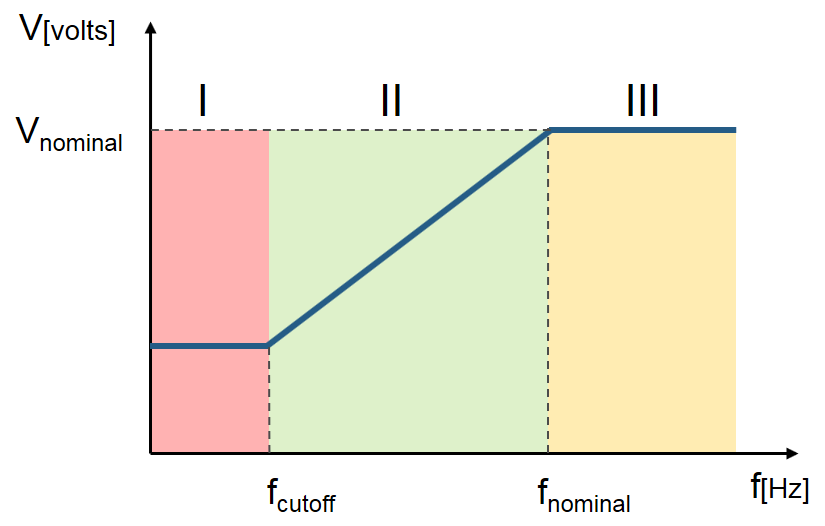
\includegraphics[width=8cm]{uf}}
		\caption{ U/f karakterisztikája}		
	\end{figure}
	
	\pagebreak
	
	Az (1.) ábra alapján az U/f karakterisztikát három részre tudjuk osztani.
	
	\begin{itemize}
		\item Az \textbf{I. tartományban} csak a stator oldali ellenálláson esik feszültség, a tényleges forgási sebesség elhanyagolhatónak tekinthető \textbf{( 0 - 5Hz )}.
		\item A \textbf{II. tartomány} lineárisnak tekinthető, melyben a maximális frekvencia értéke megegyezik a motor nominális frekvenciájával \textbf{( 5 - 60Hz )}. A lineáris tartományban a feszültség meghatározása az egyenes egyenletéből történik ($f_{cutoff} = f_{min}$).
		\item  A \textbf{III. rész a mezőgyengítési tartomány}, ahol már csak a frekvencia növelhető. \textbf{(60 - 120 Hz )}
	\end{itemize}
	
	Az feszültség amplitúdó meghatározása az egyenes egyenletének megfelelően az alábbi módon történik.
	\begin{align}
		& y = mx + b \\
		& U_{amp} = \frac{U_{nom} - U_{min}}{f_{nom} - {f_{min}}}\cdot (f_{ref} -f_{min} ) + U_{min}
	\end{align}
	A fázisszöget, a referencia frekvenciából számolt szögsebesség integrálásából kapjuk. A diszkrét idejű integrálást Forward - Euler alkalmazásával valósítottam meg, és az alábbi egyenlet mutatja.
	\begin{align}
	& \Theta[k] = 2 \cdot \pi \cdot f_{ref} \cdot T_s + \Theta[k-1]
	\end{align}
	
	Az amplitúdó és szög meghatározása után, több fajta módon lehet a fázisfeszültségeket legenerálni, számolhatunk három fázisra, $\alpha - \beta$ és D - Q koordináta-rendszerben. Három fázisra megadva a feszültségek az alábbi módon írhatóak fel.
	
	\begin{align}
		& U_U = U_{amp}  \cdot \sin \Pbracket{ \Theta } \\
		& U_V = U_{amp}  \cdot \sin \Pbracket{ \Theta + \frac{-2\pi}{3}} \\
		& U_W = U_{amp}  \cdot \sin \Pbracket{ \Theta + \frac{2\pi}{3}}
	\end{align}
	
	\pagebreak
	\section{U/f szabályzás Simulink implementációja}
	
	\begin{figure}[!htb]
		\centering
		\label{uf_full}
		\tcbox{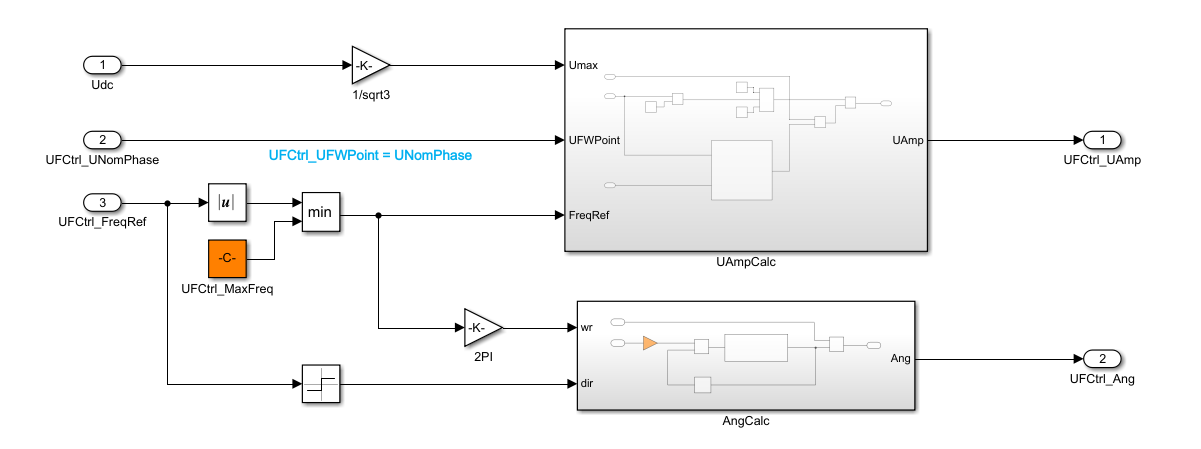
\includegraphics[width=10.7cm]{uf_full}}
		\caption{Teljes U/f szabályzás implementációja}		
	\end{figure}
	
	\begin{figure}[!htb]
		\centering
		\label{uf_amp}
		\tcbox{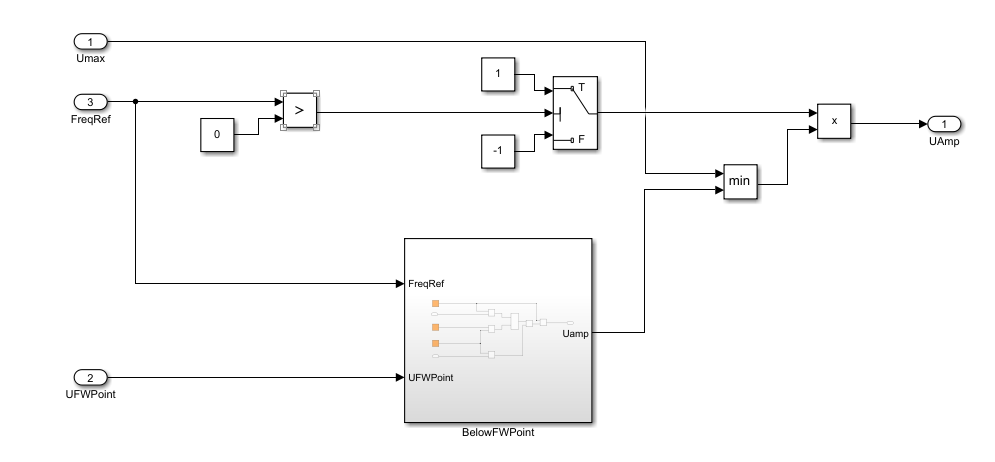
\includegraphics[width=10.7cm]{uf_amp}}
		\caption{Feszültség amplitúdó meghatározásának implementációja}		
	\end{figure}
	
	\begin{figure}[!htb]
		\centering
		\label{uf_lin}
		\tcbox{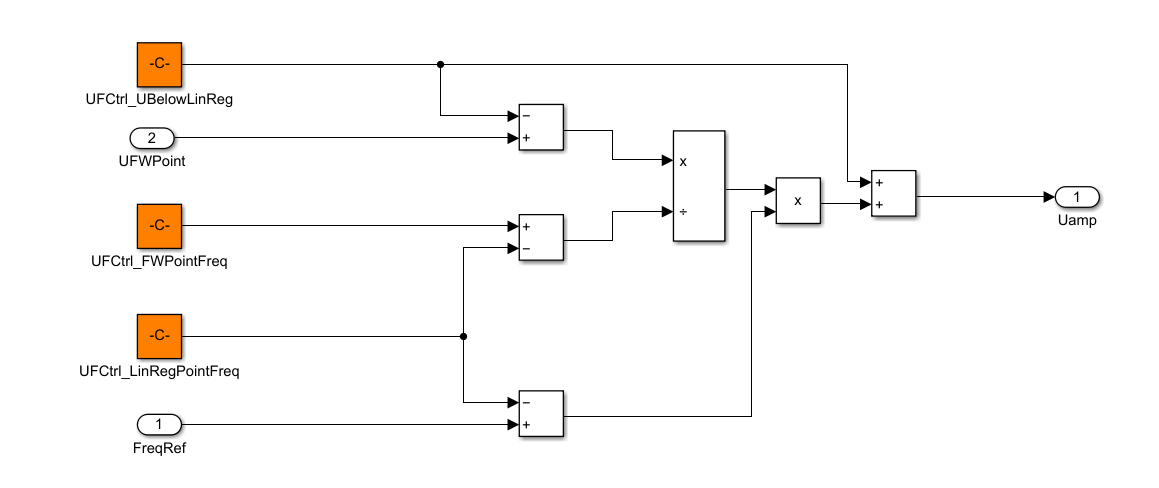
\includegraphics[width=10.7cm]{uf_lin}}
		\caption{Lineáris szakasz implementációja}		
	\end{figure}
	
	\begin{figure}[!htb]
		\centering
		\label{uf_ang}
		\tcbox{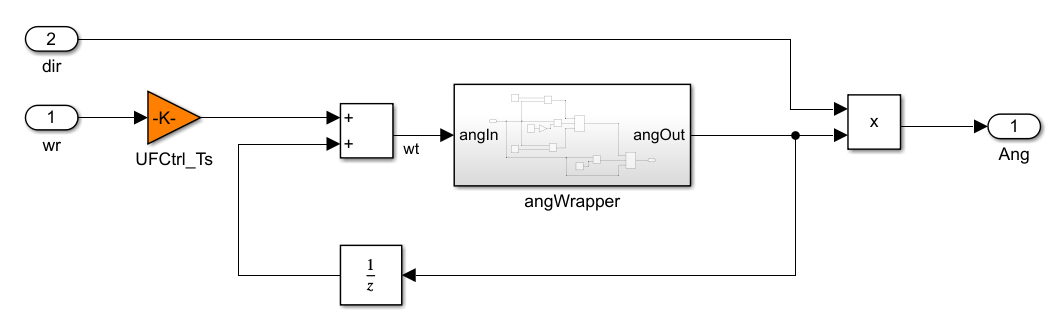
\includegraphics[width=10.7cm]{uf_ang}}
		\caption{Fázis szög meghatározása integrálással}		
	\end{figure}
	
	
	\pagebreak
	\pagebreak
	
	\section{Sebességszabályzó modell bemutatása}
	
	\begin{figure}[!htb]
		\centering
		\label{uf_invside}
		\tcbox{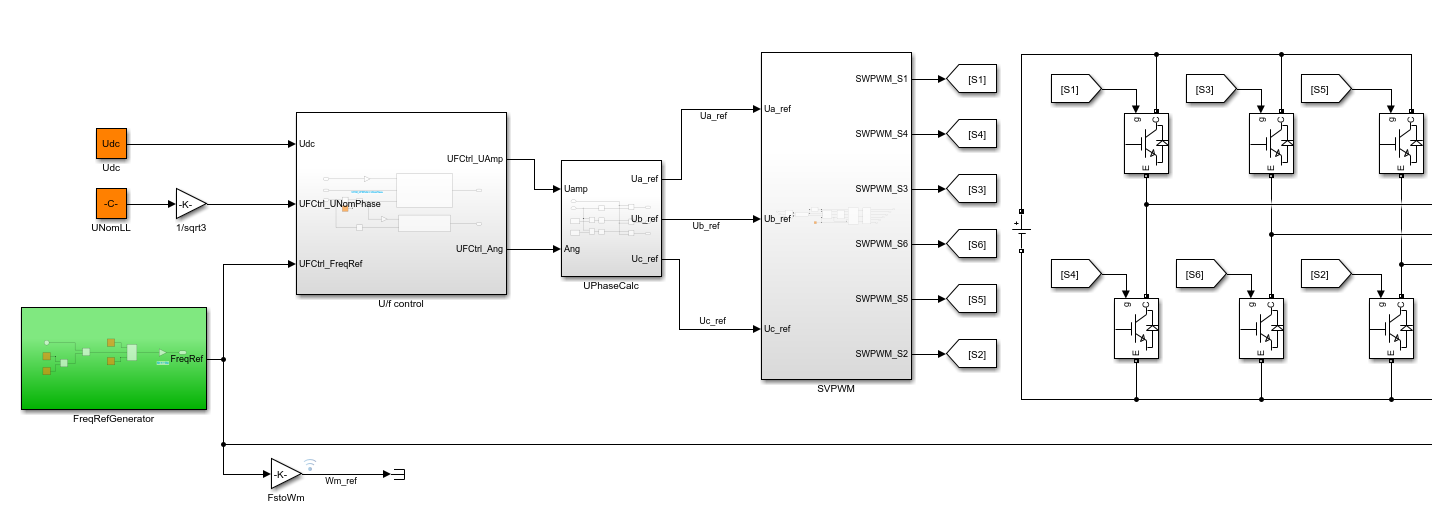
\includegraphics[width=14 cm]{uf_invside}}
		\caption{Inverter oldal implementációja}		
	\end{figure}
	
	Az inverter oldalon látható az U/f kontrol magába foglalja:
	\begin{itemize}
		\item  \textbf{FreqRefGenerator} : Referencia frekvencia "léptető" 0-120 Hz-es intervallumon 20Hz-es lépésközzel
		\item \textbf{U/f control} : Frekvencia - feszültség amplitúdó szabályzás
		\item \textbf{UPhaseCalc} : Háromfázis számításására szolgál ($U_{amp}$, $\Theta$ )
		\item \textbf{SWPWM} : Hexagonos térvektor modulációval megvalósított invertervezérlés
		\item \textbf{Kétszintű inverter Simscape modell}
	\end{itemize}
	
	Fontos megjegyezni hogy az álltalunk elvárt mechanikai szögesebbéget a \textbf{${Wm}_{ref}$} fogja szolgáltatni.
	Az itt felhasznált motorparaméterek :
	\begin{itemize}
		\item \textbf{$U_{dc}$} : DC feszültség forrás
		\item \textbf{$U_{nom_{L-L}}$} : Nominális vonalifeszültség
	\end{itemize}
	 
	\pagebreak
	\begin{figure}[!htb]
		\centering
		\label{uf_motorside}
		\tcbox{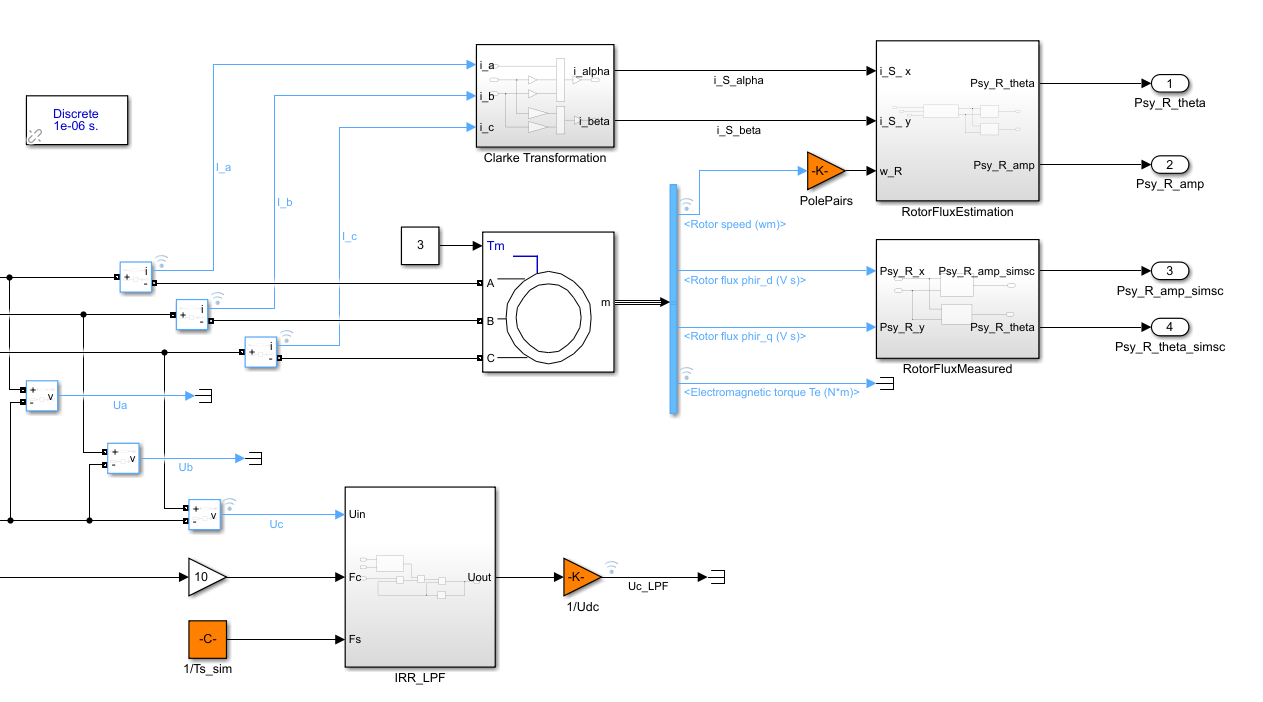
\includegraphics[width=14 cm]{uf_motorside}}
		\caption{Motor oldal implementációja}		
	\end{figure}
	
	 A motor oldal magába foglalja:
	 \begin{itemize}
	  \item \textbf{Simscape aszinkron gép} : Közvetlenül mérhetjük rajta a mechanikai szögsebességet ($Wm$)
	  \item \textbf{RotorfluxMeasured}: Motor közvetlen méréséből kapott rotorfluxus amplitúdót és szöget szolgáltatja. ($|\Psi_{R}|$ - , $\Theta_{\Psi_{R}}$ - simsc)
	  \item \textbf{RotorfluxEstimator}: Számolt rotorfluxus amplitúdót és szöget szolgáltatja.($|\Psi_{R}|$, $\Theta_{\Psi_{R}}$)
	  \item \textbf{Clarke transzformáció} : Háromfázisú időben változó rendszert, kétfázisú rendszerré egyszerűsít.
	 \end{itemize} 
	
	\section{ Modell tesztelése }
	
	Az U/f szabályzás tesztelését, egy nyílt hurkú szabályzásban (open-loop) valósítottam, melyben egy kétszintű invertert irányít, amely meghajtja a rákapcsolt aszinkron gépet.
	A rendszer bemenetét a feszültség frekvenciája képezi, 0 - 120 Hz közötti tartományon, mely 20Hz-el növekszik fix időközönként.
	
	\pagebreak
	\textbf{CÉL}: Mért és számolt értékek összehasonlítása
	\begin{itemize}
		\item \textbf{Mechanikai szögsebesség} : $Wm_{ref}$ -$Wm$
		\item \textbf{Rotorfluxus amplitúdó} : $|\Psi_{R}|$ - $|\Psi_{R}|_{simsc}$
		\item \textbf{Rotorfluxus szög} : $\Theta_{\Psi_{R}}$ - ${\Theta_{\Psi_{R}}}_{simsc}$
	\end{itemize}
	
	\begin{figure}[!htb]
		\centering
		\label{uf_wm}
		\tcbox{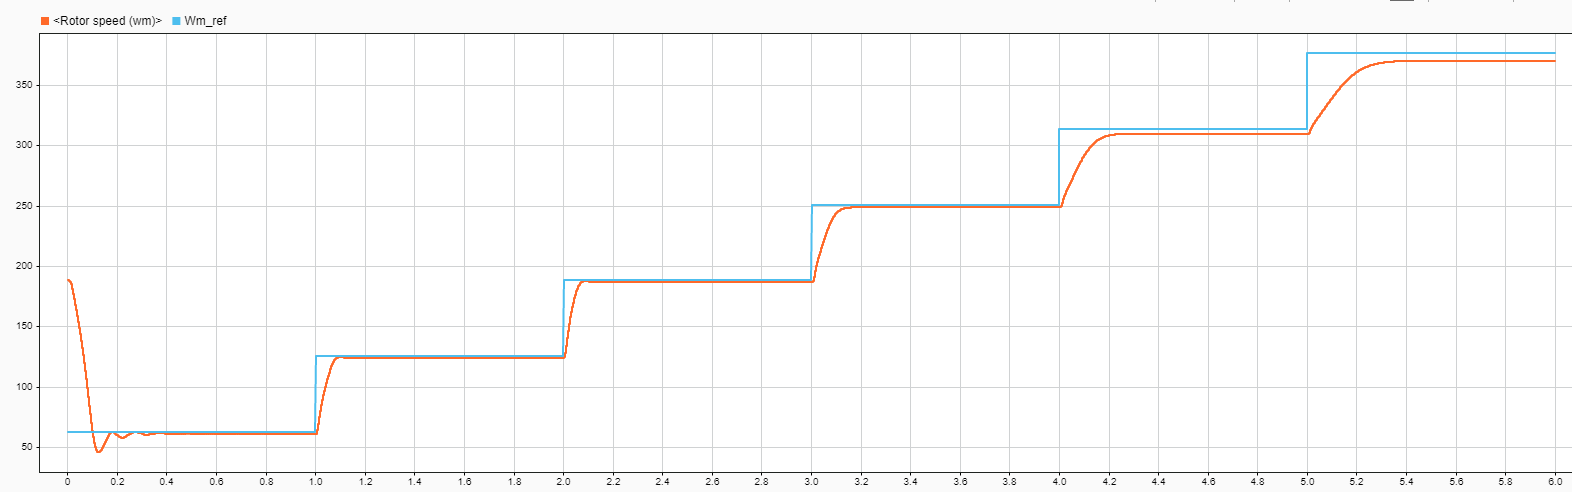
\includegraphics[width=13.2cm]{uf_wm}}
		\caption{ Mechanikai sebesség összehasonlítása ($Wm_{ref}$ -$Wm$)}		
	\end{figure}
	
	\begin{figure}[!htb]
		\centering
		\label{uf_flux}
		\tcbox{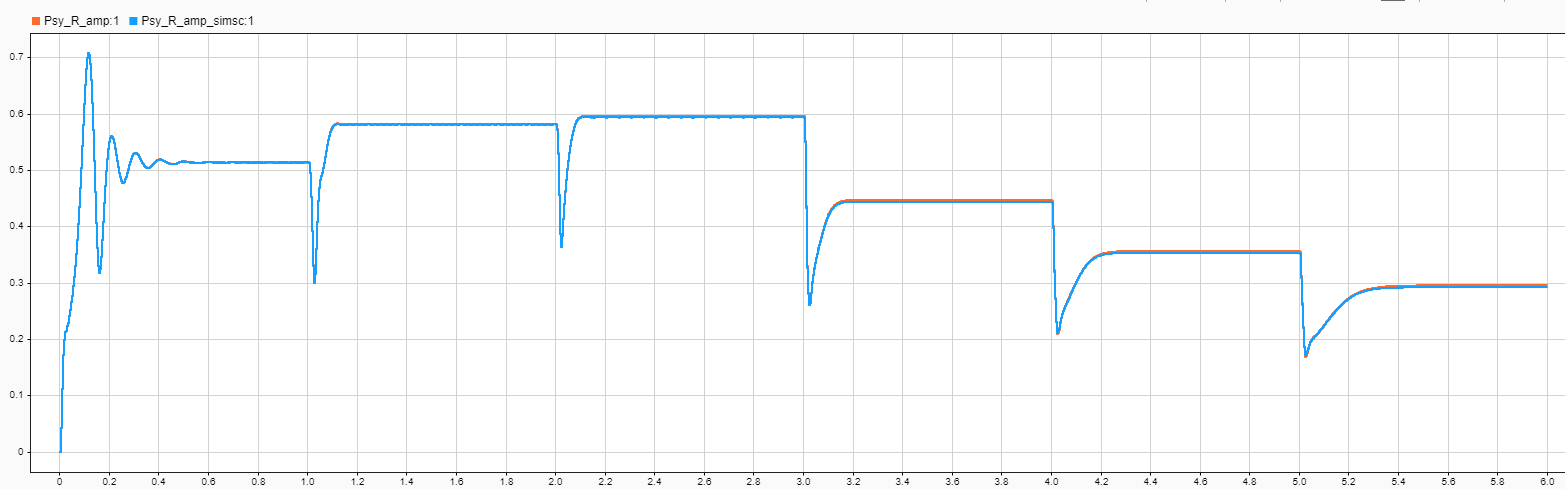
\includegraphics[width=13.2cm]{uf_flux}}
		\caption{ Rotorfluxus amplitúdó összehasonlítása ($|\Psi_{R}|$ - $|\Psi_{R}|_{simsc}$)}		
	\end{figure}
	
	\begin{figure}[!htb]
		\centering
		\label{uf_ang2}
		\tcbox{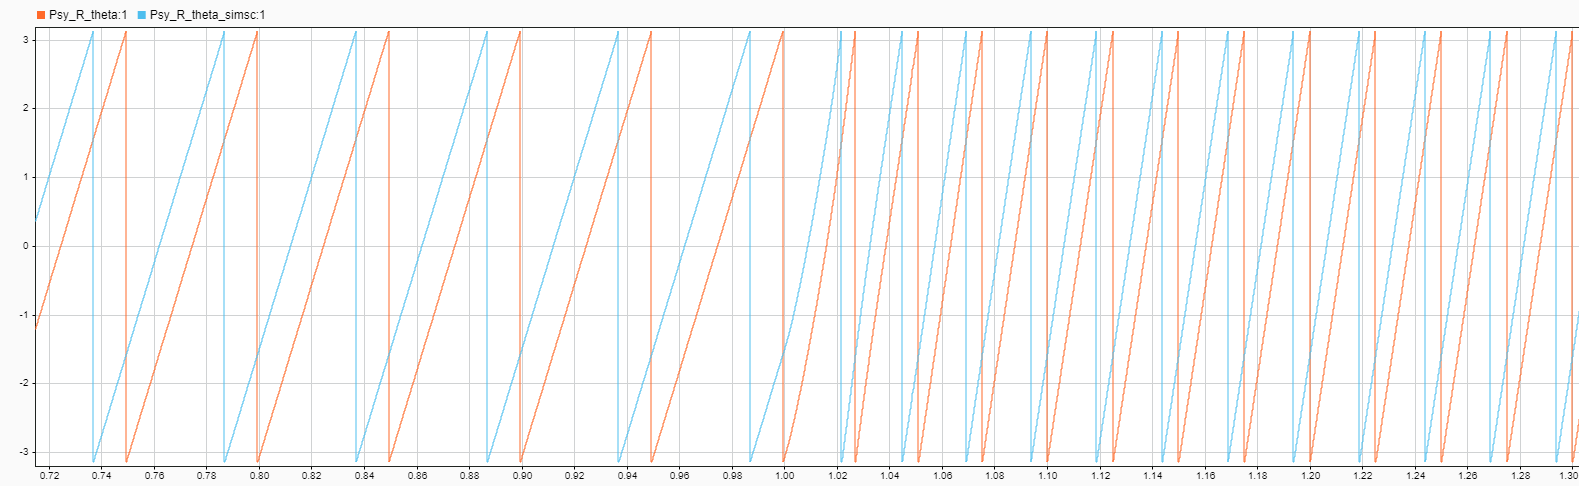
\includegraphics[width=13.2cm]{uf_ang2}}
		\caption{ Rotorfluxus szög összehasonlítása ($\Theta_{\Psi_{R}}$ - ${\Theta_{\Psi_{R}}}_{simsc}$)}		
	\end{figure}
	
	
	A (8.) és (9.) ábrát tanulmányozva jól látható, hogy mind a mechanikai sebesség, mind a rotorfluxust tekintve, kisebb lengést követően beállnak, a referencia értékre. A fluxus amplitúdó tekintetében megfigyelhető, hogy 60 Hz után csökken. Ez annak köszönhető, hogy mezőgyengítési tartományban a fluxusképző komponens, vagyis a D-irányú áram csökken. A (10.) ábrán látható hogy a rotorfluxus szög tekintetében egy 90 fokos eltérés van a mért és a számolt értékek között. Ez lényegében a D-Q koordináta-rendszer orientációjának tudható be (motor modell másképp orientálja a D-Q koordináta rendszert). Mivel ez az eltérés konstans, így a szög számítását is helyesnek tekintjük. Összességében elmondhatjuk, hogy az U/f szabályzás jól működik, valamint a tervezett fluxusbecslő és invertervezérlő komponens is az elvártnak megfelelően működik.
	

	\pagebreak
\end{document}